\section{System Overview}
The system shown in \figref{fig:systemoverview} are our current vision for the system.

\begin{figure}[h!]
  \centering
    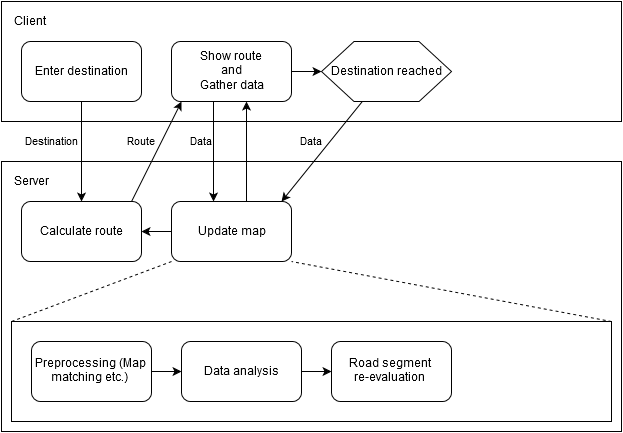
\includegraphics[width=1\textwidth]{figures/system-overview.png}
    \caption{A course grained system overview.}
    \label{fig:systemoverview}
\end{figure}

The flowschart shows how the user inputs their destination at the start. Which then is sent to a central server together with the source start address. Ther server then uses the data to calculate a route for the request. The route is then sent back to the user, while driving the user will send data back about the drive, this will be the GPS points of the route. This information is then processed and analyzed to check if traffic conditions are as they are supposed to be. If there are signs of abnormalities, this information can be used to recalculate routes for all the drivers which are passing through a that given segment. 